%-*- coding=utf-8 -*-
\documentclass[UTF8]{ctexart}

\usepackage{geometry}
\usepackage{graphicx}
\usepackage{listings}
\usepackage{algorithm}
\usepackage{color}

\usepackage{algorithmic}
\usepackage[colorlinks,linkcolor=blue]{hyperref}

\definecolor{dkgreen}{rgb}{0,0.6,0}
\definecolor{gray}{rgb}{0.5,0.5,0.5}
\definecolor{mauve}{rgb}{0.58,0,0.82}
\lstset{ %
    aboveskip=3mm,
    belowskip=3mm,
    showstringspaces=false,
    columns=flexible,
    basicstyle={\small\ttfamily},
    numbers=left,
    numberstyle=\tiny\color{gray},
    keywordstyle=\color{blue},
    commentstyle=\color{dkgreen},
    stringstyle=\color{mauve},
    breaklines=true,
    breakatwhitespace=true,
    tabsize=3
}
\geometry{left=3.18cm,right=3.18cm,top=2.54cm,bottom=2.54cm}
\pagestyle{plain}   
% \usepackage{booktabs}
% \usepackage{subfigure}
\usepackage{setspace}
\date{}
\begin{document}

\begin{center}
    \quad \\
    \quad \\
    \huge  assignment2 report
\end{center}
\vskip 3.5cm

\begin{center}
    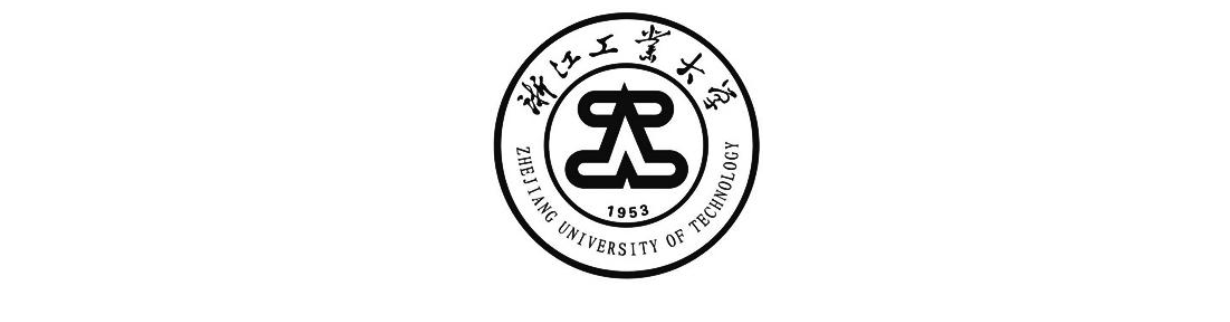
\includegraphics[scale=0.6]{../img/logo.png}
\end{center}
\vskip 4.5cm

\begin{quotation}
    \songti \fontsize{15}{15}
    \doublespacing
    \par\setlength\parindent{6.5em}
    \quad

    学\hspace{0.61cm} 院:\underline{\quad 计算机科学与技术学院、软件学院}

    专\hspace{0.61cm} 业:\underline{\qquad 软件工程(中外合作)\qquad\qquad  }

    学生姓名:\underline{\qquad\qquad\qquad 李肖 \qquad\qquad\qquad\qquad }

    学\hspace{0.61cm} 号:\underline{\qquad\qquad 202003340111 \qquad\qquad\qquad}

    \vskip 1cm
    \centering
    2022年11月26日
\end{quotation}

\newpage

\section{算法解释}
\subsection{冒泡排序}
冒泡排序的基本思想是:通过对待排序序列从前向后(从下标较小的元素开始),
依次比较相邻元素的值,若发现逆序则交换,使值较大的元素逐渐从前移向后部,
就象水底下的气泡一样逐渐向上冒。这样,每一趟会将最小的元素“浮”到顶端,最终达到完全有序。

\subsection{归并排序}
归并排序是建立在归并操作上的一种有效的排序算法,该算法是采用分治法
将已有序的子序列合并,得到完全有序的序列;即先使每个子序列有序,再使子序列段间有序。

\section{伪代码}
\subsection{冒泡排序}
\begin{algorithm}
    \caption{Bubble sort}
    \label{alg3}
    \begin{algorithmic}[1]
        \REQUIRE $n$,$a[1..n]$
        \ENSURE 排序后的序列$a[1..n]$

        \FOR {$i \gets 0$; $i < n$; $i++$ }
        \FOR {$j \gets 0$; $j < n - i - 1$; $j++$ }
        \IF {A[j] > A[j+1]}
        \STATE \textit{swap} (A[j], A[j+1])
        \ENDIF
        \ENDFOR
        \ENDFOR
    \end{algorithmic}
\end{algorithm}

\subsection{归并排序}
\begin{algorithm}
    \caption{Merge Sort}
    \begin{algorithmic}[1]
        \REQUIRE $n$,$a[1..n]$
        \ENSURE 排序后的序列$a[1..n]$
        \STATE \textbf{Function} \textit{mergeSort}($a[1..n]$)
        \IF {$n > 1$}
        \STATE $m \gets \lfloor n/2 \rfloor$
        \STATE $a_1 \gets mergeSort(a[1..m])$
        \STATE $a_2 \gets mergeSort(a[m+1..n])$
        \STATE $a \gets merge(a_1, a_2)$
        \ENDIF
        \RETURN $a$
        \STATE \textbf{END}
    \end{algorithmic}
\end{algorithm}

\newpage
\section{理论时间分析}
\subsection{冒泡排序}
\[f(n) = n ^ 2 + n\]
\subsection{归并排序}
\[f(n) = n \log n + n\]

\vskip 1cm

\newpage
\section{实验时间结果}

\begin{lstlisting}[numbers=none]
n = 10 ^ 0
Bubble sort:

real    0m0.089s
user    0m0.001s
sys     0m0.001s

Merge sort:

real    0m0.091s
user    0m0.001s
sys     0m0.001s

----------------------------
n = 10 ^ 1
Bubble sort:

real    0m0.084s
user    0m0.001s
sys     0m0.001s

Merge sort:

real    0m0.092s
user    0m0.001s
sys     0m0.001s

----------------------------
n = 10 ^ 2
Bubble sort:

real    0m0.090s
user    0m0.001s
sys     0m0.001s

Merge sort:

real    0m0.091s
user    0m0.001s
sys     0m0.001s

----------------------------
n = 10 ^ 3
Bubble sort:

real    0m0.095s
user    0m0.008s
sys     0m0.001s

Merge sort:

real    0m0.094s
user    0m0.002s
sys     0m0.001s

----------------------------
n = 10 ^ 4
Bubble sort:

real    0m0.495s
user    0m0.411s
sys     0m0.002s

Merge sort:

real    0m0.090s
user    0m0.014s
sys     0m0.001s

----------------------------
n = 10 ^ 5
Bubble sort:

real    0m39.558s
user    0m39.078s
sys     0m0.115s

Merge sort:

real    0m0.670s
user    0m0.181s
sys     0m0.004s

----------------------------
\end{lstlisting}

\section{回答问题}
\textbf{问题:}At what input size do you consider the time
required for initialization to be negligible in relation
to the total running time of the algorithm?

\textbf{回答:} 初始化数据需要 n 次操作,在 n 比较小的时候 $n ^ 2$ 和 $ n ^ log n$和 $n$ 的差距不大,
需要考虑初始化数据的时间,但是当 n 很大的时候,初始化数据的时间可以忽略不计。

\section{理论时间和实验时间的比较}
可以看到在上面的时间中,归并排序的运行时间增长非常缓慢,而冒泡排序的运行时间在 n 成为 $10^5$ 后增长非常快,
这是因为归并排序的时间复杂度是 $n \log n$,而冒泡排序的时间复杂度是 $n ^ 2$,
所以归并排序的运行时间增长非常缓慢,而冒泡排序的运行时间增长非常快。

\section{代码实现}
\subsection{冒泡排序}
\lstinputlisting[language=C++]{../../code/bubble.cpp}
\subsection{归并排序}
\lstinputlisting[language=C++]{../../code/merge.cpp}

\end{document}